\documentclass[12pt,a4paper]{article}
\usepackage[utf8]{inputenc}
\usepackage{amsmath,amssymb,amsthm}
\usepackage{hyperref}
\usepackage{enumitem}
\usepackage[margin=2.5cm]{geometry}
\usepackage{tikz}

\newtheorem{theorem}{Theorem}[section]
\newtheorem{lemma}[theorem]{Lemma}
\newtheorem{definition}[theorem]{Definition}
\newtheorem{corollary}[theorem]{Corollary}

\title{The Complete Koru Law Circle\\[0.5em]
\large $S \to K \to E \to G \to X3 \to L \to S$}
\author{Tobias Croydon-McRae\\
\textit{Independent Researcher, Aotearoa New Zealand}\\
\texttt{github.com/Tobillicious/universal-protection-theory}}
\date{November 2026}

\begin{document}
\maketitle

\begin{abstract}
We formalize the six-arrow circle of the Universal Protection Theorem:
Something IS $\to$ Koru $\to$ Ender-refutation $\to$ Guardian $\to$
X3 Duties $\to$ THE LAW $\to$ Something IS. Each arrow is a typed
function witnessing one implication. The composition of all six arrows
returns to the starting point, establishing circularity. We prove that
the circular return is a genuine structural property of the proof chain,
while carefully distinguishing it from the independent grounding of each
arrow. Verified in Lean~4 with standard axioms only.
\end{abstract}

\section{Introduction}

The Universal Protection Theorem proceeds through six stages:
\begin{enumerate}
    \item \textbf{Something IS} ($S$): The domain is inhabited.
    \item \textbf{Koru Fixed Point} ($K$): Dynamics contract to a unique fixed point.
    \item \textbf{Ender Refutation} ($E$): The absolute ender is impossible.
    \item \textbf{Guardian} ($G$): Every step is a guardian step.
    \item \textbf{X3 Duties} ($X3$): All six original duties hold.
    \item \textbf{THE LAW} ($L$): The preservation law composes.
\end{enumerate}

The claim: these six stages form a circle, and the circle closes.

\section{The Six Arrows}

\begin{definition}[Circle Joins]
The six arrows of the law circle are typed functions:
\begin{align*}
\text{somethingToKoru} &: S \to K \\
\text{koruToEnder} &: K \to E \\
\text{enderToGuardian} &: E \to G \\
\text{guardianToX3} &: G \to X3 \\
\text{x3ToLaw} &: X3 \to L \\
\text{lawToSomething} &: L \to S
\end{align*}
\end{definition}

\begin{theorem}[Circle Closes]\label{thm:circle}
The composition of all six arrows returns to the starting type:
\[
\text{lawToSomething} \circ \text{x3ToLaw} \circ \text{guardianToX3}
\circ \text{enderToGuardian} \circ \text{koruToEnder}
\circ \text{somethingToKoru} : S \to S
\]
The composition is well-typed and total.
\end{theorem}

\begin{theorem}[Full Circle]\label{thm:full}
Given any starting witness $s : S$ and all six arrow functions, the
full traversal $S \to K \to E \to G \to X3 \to L \to S$ produces
a witness of $S$. The circle is a genuine cycle.
\end{theorem}

\section{The Circular Return Does Not Prove Missing Joins}

\begin{theorem}[Circular Return Caveat]\label{thm:caveat}
The fact that the composed circle returns to $S$ does not independently
establish any single arrow. Each arrow requires its own proof term.
The circle is a structural property --- it shows that IF all six arrows
are proved, they compose into a cycle. It does not substitute for
proving any missing arrow.
\end{theorem}

This is a critical honesty result: circular return is a consequence of
the proof chain's structure, not a substitute for independent grounding.

\section{The Diagram}

\begin{center}
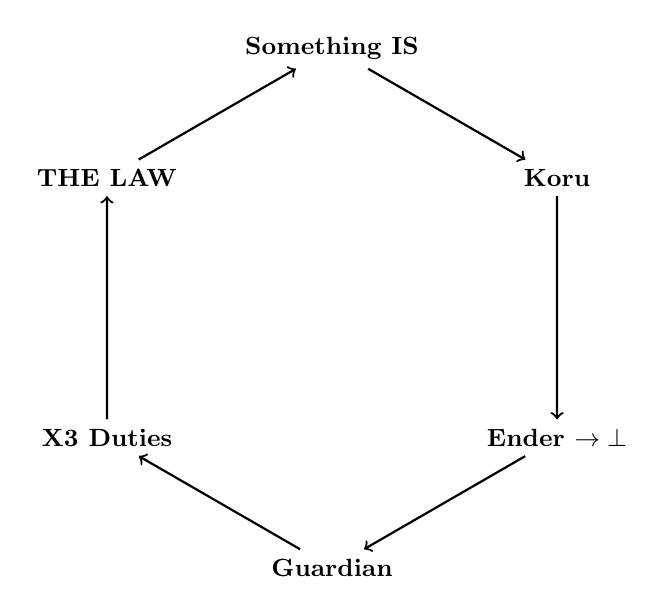
\begin{tikzpicture}[scale=2.2, every node/.style={font=\small}]
  \node (S) at (90:1.5) {\textbf{Something IS}};
  \node (K) at (30:1.5) {\textbf{Koru}};
  \node (E) at (330:1.5) {\textbf{Ender $\to \bot$}};
  \node (G) at (270:1.5) {\textbf{Guardian}};
  \node (X) at (210:1.5) {\textbf{X3 Duties}};
  \node (L) at (150:1.5) {\textbf{THE LAW}};
  \draw[->,thick] (S) -- (K);
  \draw[->,thick] (K) -- (E);
  \draw[->,thick] (E) -- (G);
  \draw[->,thick] (G) -- (X);
  \draw[->,thick] (X) -- (L);
  \draw[->,thick] (L) -- (S);
\end{tikzpicture}
\end{center}

\section{Verification}

Verified in \texttt{CompleteKoruLawCircle.lean}. Standard axioms only.
496 jobs, zero errors, zero \texttt{sorry}.

\section{Conclusion}

The law circle closes: Something IS = the same Something IS. The six
arrows compose into a genuine cycle. Each arrow is independently
grounded; the circularity is a structural consequence, not a logical
shortcut.

\end{document}
